\section{An\'alisis de entrop\'ia}


\indent Para este punto decidimos tomar como s\'imbolos de la fuente de informaci\'on a las direcciones IP de los nodos de una red de hogar.
Como modelo vamos a analizar los datos de diferentes maneras:

\subsubsection{Primera red (6 horas de capturas de paquetes):}

\begin{itemize}
 \item  IPs que realizaron consultas ARP:
\end{itemize}

\begin{tabular}{|l|l|l|l|l|}
  \hline
  S\'imbolo & Consultas & Probabilidad & Informaci\'on \\
  \hline
  192.168.0.105 & 99 & 0.0947368421053 & 3.39993060689 \\
  \hline
  192.168.0.104 & 28 & 0.0267942583732 & 5.22193230491 \\
  \hline
  192.168.0.1 & 448 & 0.428708133971 & 1.22193230491 \\
  \hline
  192.168.0.101 & 415 & 0.397129186603  & 1.33231970073 \\
  \hline
  192.168.0.100 & 1 & 0.000956937799043 & 10.029287227 \\
  \hline
  192.168.0.103 & 11.0 & 0.0105263157895 & 6.56985560833 \\
  \hline
  192.168.0.102 & 26 & 0.0248803827751 & 5.32884750883 \\
  \hline
  0.0.0.0 & 17 & 0.0162679425837 & 5.94182438572 \\
  \hline
\end{tabular}\\


Entrop\'ia de la fuente:\\
$H(S) = 1.82297065237$\\

\begin{figure}[h]
  \centering                                                       
          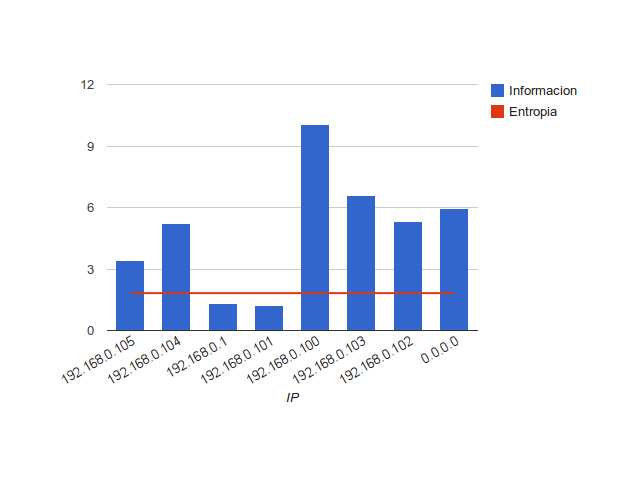
\includegraphics[width=300pt]{consultas1.png}
\end{figure}

En este caso la IP que realiz\'o m\'as consultas ARP fue 192.168.0.1 (router), \'esto es l\'ogico considerando que el router es el encargado de distribuir todo el tr\'afico de la red a los nodos correspondientes por lo que su tabla
de direcciones macs tiene que estar correctamente actualizada el mayor tiempo posible.\\\\


\begin{itemize}
 \item  IPs que respondieron consultas ARP:
\end{itemize}

\begin{tabular}{|l|l|l|l|l|}
  \hline
  S\'imbolo & Respuestas & Probabilidad & Informaci\'on \\
  \hline
  192.168.0.105 & 506 & 0.85472972973 & 0.226459790935 \\
  \hline
  192.168.0.101 & 24 & 0.0405405405405 & 4.62449086491 \\
  \hline
  192.168.0.1 & 62 & 0.10472972973 & 3.25525705524\\
  \hline
\end{tabular}\\
 
Entrop\'ia de la fuente\\
$H(S) = 0.721963466885$\\

\begin{figure}[h]
  \centering                                                       
          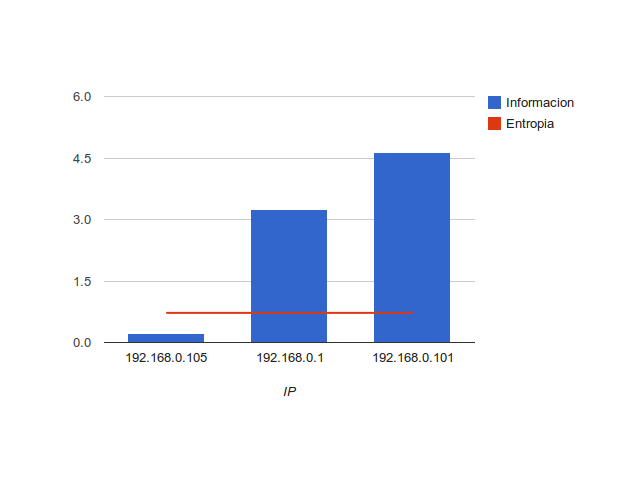
\includegraphics[width=300pt]{respuestas1.png}
\end{figure}

En este caso la IP 192.168.0.105 fue la que m\'as veces contest\'o los pedidos sobre su MAC, aumentando su probabilidad. Como se puede observar, la informaci\'on
aportada por esta IP es considerablemente m\'as baja que la aportada por las dem\'as que poseen menor probabilidad e incluso m\'as baja que la entrop\'ia de la red.\\\\\\

\begin{itemize}
 \item IPs por las que se realizaron consultas ARP:\\
\end{itemize}

\begin{tabular}{|l|l|l|l|l|}
  \hline
  S\'imbolo & Consultas & Probabilidad & Informaci\'on \\
  \hline
  169.254.37.204 & 3 & 0.00287081339713 & 8.44432472625\\
  \hline
  192.168.0.105 & 506 & 0.484210526316 & 1.04629365227\\
  \hline
  192.168.0.104 & 52 & 0.0497607655502 & 4.32884750883\\
  \hline
  169.254.255.255 & 10 & 0.00956937799043 & 6.70735913208\\
  \hline
  192.168.0.1 & 88 & 0.0842105263158 & 3.56985560833\\
  \hline
  192.168.0.101 & 30 & 0.0287081339713 & 5.12239663136\\
  \hline
  192.168.0.100 & 316 & 0.302392344498 & 1.72550647879\\
  \hline
  192.168.0.103 & 18 & 0.0172248803828 & 5.85936222553\\
  \hline
  192.168.0.102 & 22 & 0.0210526315789 & 5.56985560833\\
  \hline
\end{tabular}\\
\\ \ \\ \ \\ 
Entrop\'ia de la fuente\\
$H(S) = 1.99810125093$\\

\begin{figure}[h]
  \centering                                                       
          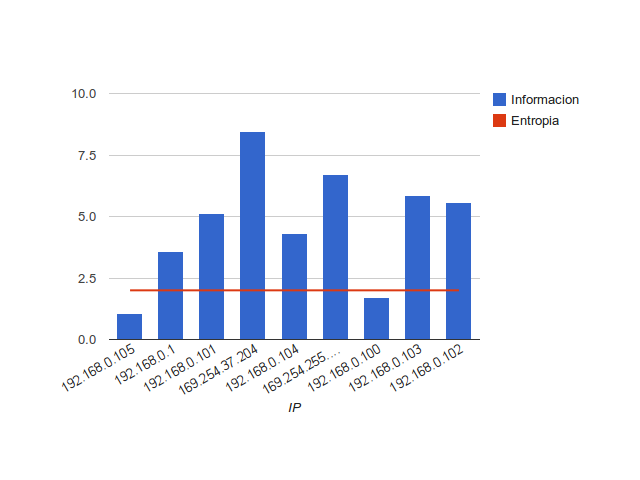
\includegraphics[width=300pt]{consultadas1.png}
\end{figure}

En este caso la IP m\'as consultada en la red fue la 192.168.0.105. Al igual que en el punto anterior por consecuencia de su alta probabilidad de aparecer en la fuente, su informaci\'on no supera a la entrop\'ia que ofrece la red.

